

\newcommand{\SYSTEM}{Mesh\xspace}

{\rmfamily
This work was previously published in ACM UIST 2020 and has been adapted for this document.
}

This chapter describe a third and final system in this dissertation that focus on supporting individual online sensemaking tasks. The two previous chapters each focused on providing global context relating to \emph{options} (Weaver in \Cref{chap:weaver}) or \emph{criteria} (SearchLens in \Cref{chap:searchlens}), and discovered important insights about users: 1) Users need to keep track of the different options that they were considering, and evaluate them under the global context (\Cref{chap:weaver}); and 2) Users often identify criteria from data and need to evaluate their options based on different criteria. Combining these insights, this chapter focus on a system that can provide holistic support for product comparison, allowing users to both keep track of their options and criteria, as well as keeping track of their personal interpretation of data to scaffold their decision making process.

While there is an enormous amount of information available online for making decisions such as choosing a product, restaurant, or school, it can be challenging for users to synthesize that information into a good decision. Information for users' many different criteria needs to be gathered from many different sources into a structure where they can be compared and contrasted. The usefulness of each criteria for differentiating potential options can be opaque to users, and evidence such as reviews may be subjective and conflicting required users to interpret each under their personal context. We introduce \SYSTEM, which scaffolds users in iteratively building up a better understanding of both their criteria and options by evaluating evidence gathered across sources in the context of consumer decision making. \SYSTEM bridges the gap between decision support systems and exploratory search, changing the cost structure to provide an increasing payoff with greater user investment. Our lab and field deployment studies found evidence that it significantly reduces the costs of gathering and evaluating evidence and scaffolds decision making through personalized criteria allowing our participants to gain deeper insights from data.





\begin{figure*}
    \centering
    \textcolor{gray}{\frame{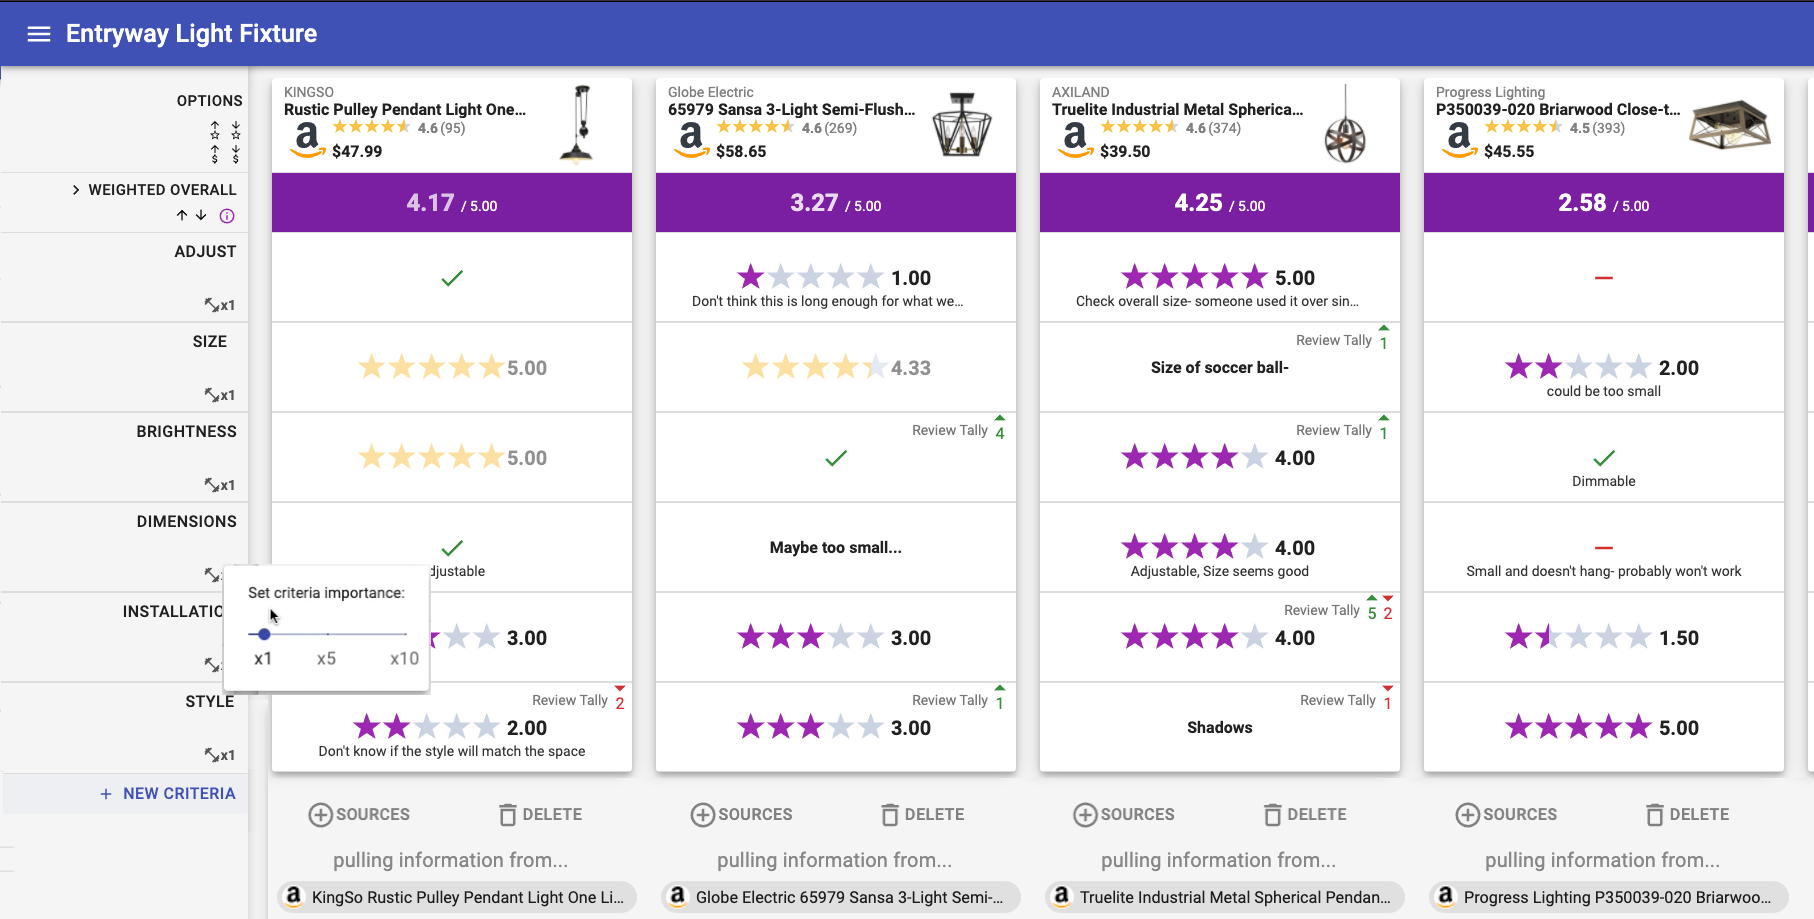
\includegraphics[width=1.0\textwidth]{Chapters/Mesh/figures/TableView3.png}}}
    \caption[The Table View for \SYSTEM]{The Table View. Users can create Option Columns by importing Amazon project pages opened in their browser tabs, and create Criteria rows to see the average review ratings that mentioned each criteria across their options (in yellow). To see explore the reviews more deeply, users can click on the criteria to see the Evidence View (shown in Figure~\ref{fig:EvidenceView}), where users can overwrite the default Amazon ratings with their own (in purple) based on their own interpretation of data. To prioritize the criteria, users can also adjust the weight to see an weighted average rating across their criteria for each option. This image is an actual project made by P05 in the field deployment study.}
    \label{fig:TableView}
\end{figure*}

\section{Introduction}

Whether figuring out which products to purchase or where to eat in an unfamiliar city, consumers today have instant access online to enormous amounts of information on which to base their decision. However, users could also be overwhelmed by the number of options, the criteria they should use to compare the options, and the number of information sources to collect evidence from \cite{simon1996designing,schwartz2004paradox}. For example, the electronics section of Amazon alone contained more than 1.3 million reviews in 2013 \cite{mcauley2013hidden}, and Yelp has accumulated more than 200 million reviews \cite{Yelpcum70:online}. Research in consumer behavior has found such reviews to be a major factor in online decision making \cite{gan2012helpfulness,mudambi2010research}. Online information has the potential to help consumers make more informed decisions about how well each option satisfies their various criteria \cite{de2016navigating}. For example, a coffee drinker looking to buy a new espresso machine might read reviews aiming to evaluate how easy it is to use for a novice barista, how well it steams milk, how likely it is to break down, and so on. On the other hand, online reviews can also be messy, biased, subjective and scattered across many sources \cite{hoch1986consumer, racherla2012perceived,zhang2012human,chen2015tripplanner}, requiring users to interpret each piece of evidence based on their personal context \cite{shugan1980cost}. The highly bimodal skew of review ratings can lead to compression of ratings in a narrow band \cite{hu2009overcoming}, and the increasing number of fake reviews (which now may be in the majority for some categories such as electronics and beauty \cite{Howmerch65:online}) mean that solely relying on automatic aggregation such as average ratings or summarizations can be risky or uninformative. Automated approaches to addressing these issues, such as aspect extraction \cite{manek2017aspect,yu2011aspect}, review summarization \cite{hu2004mining,li2010structure}, and direct recommendation \cite{bobadilla2013recommender}, can be insufficient due to the long tail of usage contexts \cite{bernstein2012direct}, the need for nuanced contextualization when reading reviews \cite{chang2019searchlens}, and the challenge of discovering and learning new criteria along the way.

Consumers doing this task manually must go through the various reviews and information sources, pulling together scattered information, learning about what criteria are useful for picking or ruling out options, evaluating evidence on those criteria, keeping track of their judgments, and weighing them depending on what's most important to them to make a final decision. To assist with the process, consumers utilize techniques such as building comparison tables with spreadsheets or notepads. However, transferring information between information sources and spreadsheets or notepads can be prohibitively time-consuming \cite{altmann2004task}. Furthermore, as a user encounters and adds new options, they must gather information for each of their criteria in the table in order to evaluate that feature. Similarly, encountering and adding new criteria requires gathering information for all previously added options. This iterative construction is common in new domains \cite{marchionini2006exploratory} and creates an increasing cost the more options and criteria in the table.

Instead of fully automated or manual approaches, we introduce \SYSTEM, a hybrid approach aimed at scaffolding decision making by helping users progressively build up a comparison table that reflects their personalized criteria and evaluations of evidence. \SYSTEM lowers the cost of pulling information into the table, organizing it by the user’s criteria, and helping users keep track of their judgments as they evaluate evidence. Importantly, by autofilling rows and columns when new criteria or options are added throughout the process, \SYSTEM makes adding to or changing the table stay at a constant cost as the table grows, changing the cost structure to provide an increasing payoff with greater user investment. Finally, \SYSTEM helps keep users on track by prioritizing where to look, which criteria are most important, and reflecting their current beliefs for each option through an overall weighted average.

We evaluated \SYSTEM through three user studies. We found evidence that \SYSTEM lowered interaction costs, and allowed participants to find answers to objective criteria, such as the size and capacity of coffee machines, significantly faster and more accurately. For subjective criteria, such as the ease of use of coffee machines, participants were able to produce summaries of what they learned in 20 minutes that were rated more insightful when compared to baseline participants who used Google Spreadsheets to conduct the same task. Finally, our field deployment study found participants were able to conduct their own tasks over a prolonged period of time, and described their process as organized and efficient allowing them to make confident purchases based on their own research.

\section{Related Work}

Research in consumer behavior has pointed to the difficulties users face when using online evidence to support making purchase decisions. One major challenge is that online evidence, such as consumer or expert reviews, can be subjective, biased and messy \cite{mudambi2010research,Howmerch65:online}. Furthermore, users may need to go through a each piece of evidence in order to interpret them based on their own personal context and unique goals. This process is an important factor in purchase decision making \cite{gan2012helpfulness,mudambi2010research}, but can incur high cognitive costs as the user tries to keep track of and summarizing each piece of evidence. Another major challenge is that online evidence is often scattered across many information sources due to the distributed nature of the Web. This includes product listing pages on ecommerce platforms, blog and forum posts, and consumer and expert reviews. On the one hand, having multiple information sources can help users to determine the credibility of online evidence \cite{hoch1986consumer, racherla2012perceived,zhang2012human,chen2015tripplanner}. However, cross-referencing multiple sources can be burdensome and costly \cite{o1996towards,marshall1999introducing,tashman2011liquidtext,bianchi2015designing}.


%\SYSTEM tackled these issues using two approaches. Firstly, it introduces a new way to navigate and explore online evidence by allowing users to group and connect information sources to options they want to compare, and search across them to see evidence about different options laid out. A process that otherwise would involve manually filtering multiple webpages, and switching back and forth between browser tabs. Secondly, when users examine individual pieces of evidence, \SYSTEM captured their judgments about data with minimal effort, allowing them to gradually build up a comparison table process that matched their own values and interpretation of data, and eventually use it to support making the final purchase decision.

Significant research effort has been focused on using computational approaches to support this process, using the wealth of available data for training machine learning models. One thread of research is focused on making direct product recommendations by either finding patterns from the purchase history of many users \cite{bobadilla2013recommender} and/or the description and metadata of products \cite{Lops2011ContentbasedRS}. Personalized product recommendations can potentially shortcut users' research effort but also face issues with accuracy and explainability \cite{bilgic2005explaining}. Another thread of research is focused on reducing users' effort when consuming large numbers of reviews by aggregation, such as review summarization and common criteria (aspect) extraction from reviews \cite{Howmerch65:online}. However these approaches also face issues with user trust, for example from fake reviews polluting the aggregated results or failing to support the long tail distribution of less common user needs \cite{bernstein2012direct}. Furthermore, current approaches fail to support the qualitative process of developing personalized context from subjective data that is vital to human decision making. Not unrelated, recent research has found reading consumer reviews to still play an important role in online purchase decisions \cite{gan2012helpfulness,mudambi2010research}, even though recommender systems are now widely available on ecommerce platforms. 

Another thread of research has focused on building interactive interfaces that aim to support decision making under multi-criteria and multi-options scenarios, such as faceted interfaces \cite{hearst2006design,schraefel2006mspace} and table-based decision support and visualization systems \cite{chi1997spreadsheet,rao1994table,spenke1996focus,liu2019unakite}. While these approaches allow consumers to narrow down their options efficiently by navigating to different subsets of a larger collection or investigate trade-offs between them through visualization, the majority of these work rely on pre-compiled metadata or required users to manually clip evidence across different sources. As a result, they do not support accessing criteria that require close examination of a large amount of subjective evidence (such as reviews) that are not in the form of structured metadata. For example, to get a sense of how durable an option is would typically involve consumers evaluating many unstructured reviews describing whether and how an item held up over time. In two studies closely related to our work, \cite{chen2014experiment,chen2017explaining} allowed users to build comparison tables for camera products by allowing them to pick from a list of precompiled common camera criteria and used sentiment analysis of relevant reviews as summaries across different options. While \SYSTEM also allowed users to build comparison tables with their own options and criteria, in our system users can use arbitrary search terms as their criteria instead of selecting from a common list of criteria, allowing it to support the long tail distribution of user needs \cite{bernstein2012direct}. More importantly, \SYSTEM focuses on helping individual interpret reviews under their own personal context, and overwrite the summaries generated by the system to better reflect their own views of data. This approach not provides better support for personal context, but can also allow users to recover from errors made by automated summarization approaches.

%Fundamentally, these work provided a ridged structure to support decision making based on objective data often using a single source of truth (i.e., metadata), and do not support the fluid nature of accessing subjective and unstructured evidence that is important to online product research \cite{searchlens 21 36}.

Instead of automating away the role of the user, our approach focuses on helping them scaffold their decision-making throughout the process, maximizing their ability to apply their personal context and interpretation to evidence while reducing the costs for doing so. This view unlocks a design space in which the interface supports the human in discovering and sharpening their own understanding of what criteria are important to them in the context of the options and evidence available to them; keeping track of their evaluations of that evidence for them; enabling the human to prioritize their attention to the most discriminative evidence; capturing human perceptions of value; and using those perceptions to drive a final decision that integrates values across their personal criteria. At a high level our work aimed to bridge the gap between decision support research in the literature above (which helps people make decisions by imposing a high degree of structure based on metadata or through computation) and the sensemaking process in which users are learning about the unknown unknowns to develop personalized context from unstructured data \cite{russell1993cost,marchionini2006exploratory}.

\begin{figure*}
    \centering
    \textcolor{gray}{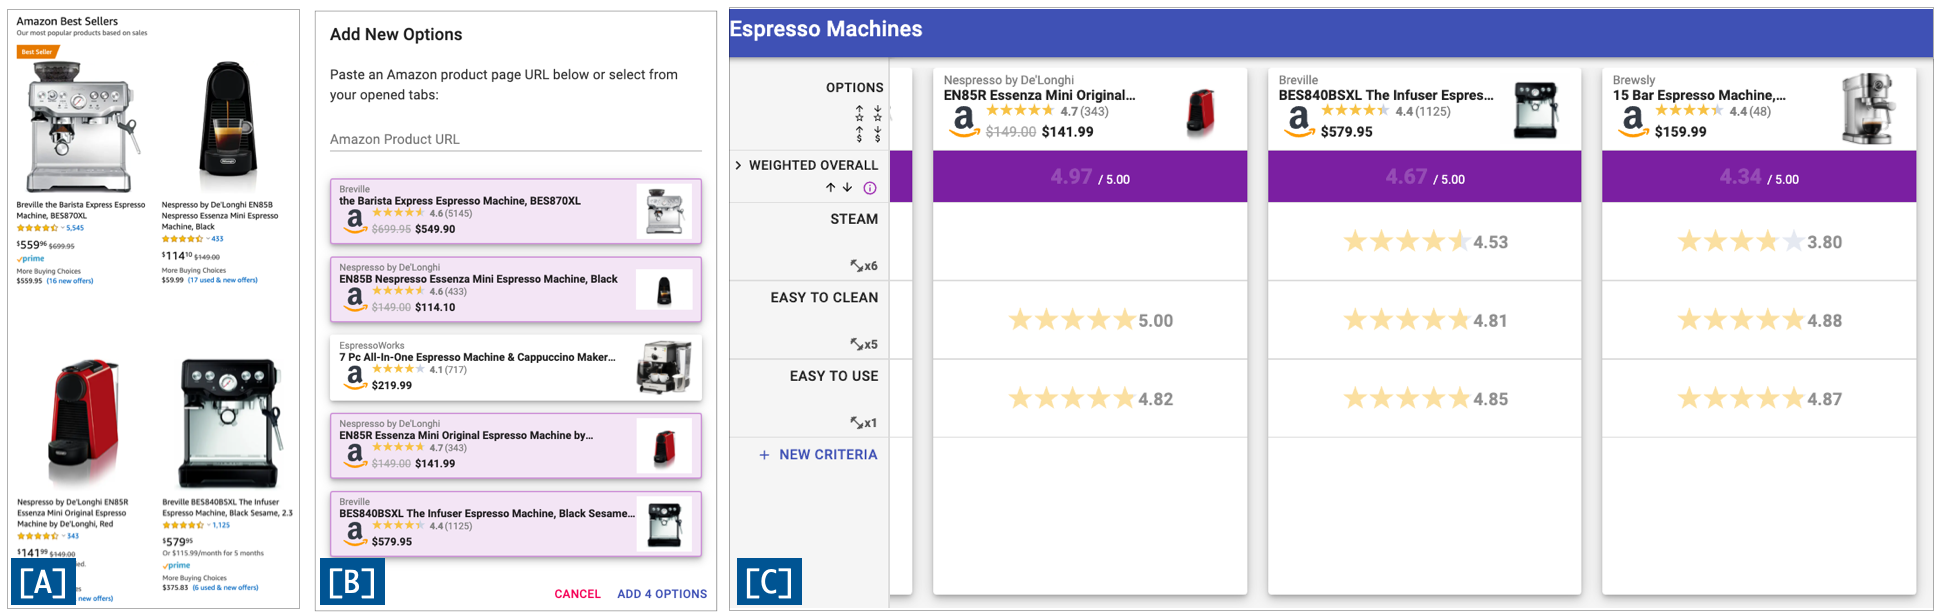
\includegraphics[width=1.0\textwidth]{Chapters/Mesh/figures/Import.png}}
    \caption[Importing tabs into \SYSTEM as product options]{Many products on Amazon are highly rated with thousands of views and it can be difficult for users to differentiate them [A]. Users can open them in browser tabs and import them into \SYSTEM to keep track of them [B]. \SYSTEM automatically fetches reviews relevant to different user criteria for each option to help characterize them [C]. Users can uncover meaningful discrepancies between options based on their own criteria. For example, here seeing a larger differences in the ``Steam'' criteria, with the first option that lack this feature returning no reviews that mentioned ``Steam''.}
    \label{fig:import}
\end{figure*}


\section{Exploratory Interviews and Design Goals}

To discover the limitations and needs of common online product research practice, we conducted preliminary interviews to inform our design goals. We recruited 30 participants (age: 3\% 19-24, 20\% 25-34, 33\% 35-40, 23\% 41-54, 20\% 55+; 22 female, 7 male, and 1 not listed) by posting on social media including Facebook, Twitter and Nextdoor, and interviewed each of them for 60 minutes.  Prior to the interviews, we generated 10 interface design mock-ups addressing various potential issues discussed in the previous sections, ranging from managing information sources to collecting evidence for purchasing decisions. We discuss these design probes in context of our discoveries below. During the interviews, we walked through each of the design mock-ups and used them as probes to see how strongly participants identified with the issues they tried to address, as well as how they reacted to the designs. We list below three of the most common recurring themes.

\subsubsection{Comparing Options with Scattered Evidence}

The most common theme mentioned by all participants was the difficulty of managing an overwhelming number of information sources and the amount of evidence scattered across them. Specifically, they pointed to how evidence for options needs to be collected across different webpages, leading to a \emph{stressful number of opened browser tabs} of ecommerce websites (such as Amazon) and expert review websites (such as CNET reviews). When comparing options, participants were especially frustrated by the high interaction cost of \emph{switching back and forth between tabs to compare options on a metric} [criteria] and that it is \emph{not easy to search for [information that mentioned] specific terms across all products}.

\subsubsection{Need for Personal Interpretation of Evidence}

Consistent with prior work, we also found reading reviews to be an important factor for supporting online shopping  \cite{gan2012helpfulness,mudambi2010research}. At the same time, participants felt overwhelmed by the amount of evidence they needed to process in order to confidently make purchase decisions, but were unenthusiastic about designs centered around automating the process. For example, one design had users answer questions about their preferences and provide personalized product recommendations. Participants were reluctant to be convinced by an automated system, but instead saw it as a way to \emph{get some ideas or guidelines about things they should consider}; in other words, they saw it as an additional source for collecting potential options to conduct further comparison. Participants further emphasized the importance of seeing raw evidence and making their own judgments such as \emph{reading through reviews to generate a summary of their own opinion}. Participants were enthusiastic about features that would support this process, such as allowing them to easily rate and tally reviews as positive or negative, or making a summary rating from reading multiple reviews.

\subsubsection{Scaffolding Decision Making}

Participants pointed to difficulties in keeping track of their overall research, describing their process as ``\emph{erratic}'' causing them to ``\emph{go down many rabbit holes}'' and ``\emph{get lost in the weeds}.'' One main reason is the need to constantly make small and personalized judgments throughout such as interpreting how relevant a review is to their personal context, summarizing how a product fits a criteria, or deciding to keep or rule out a potential option. Participants were frustrated when ``\emph{Sometimes I can’t remember why a [product] page was kept opened and had to reread the content}.'' Currently, participants used spreadsheets, scratchpads and physical notebooks to address this \emph{when things start to get out of hand}, but they also pointed to how this process is cumbersome and only used \emph{as a last resort on important purchases}. When asked about the types of information they would typically save, participants described a mix of factual findings (such as product specifications) and their own interpretation of subjective evidence (such as ease of use as described in the reviews). Participants were enthusiastic about designs that would scaffold them in working in a more organized fashion, such as making a comparison table of options they are considering and with their own criteria and notes and being able to compare options side-by-side and ranking them.

Based on these findings uncovered through the interviews, we formulate the following design goals:

\begin{itemize}
  \setlength\itemsep{0em}

\item \textbf{D1}: Minimize effort of comparing evidence for the same criteria across different options
\item \textbf{D2}: Allow users to make their own interpretation of data and summarizing them
\item \textbf{D3}: Capture users their decisions about options and criteria throughout the process in an organized way
\end{itemize}

\section{System Design}

Motivated by the design goals uncovered by our exploratory interviews, \SYSTEM focuses on providing a more organized way to conduct research by allowing users to iteratively build up a product comparison table with their own options and criteria. 

In a standard spreadsheet, people have to start with a blank table and switch back and forth between information sources to fill out everything manually. In contrast, our system provides an increasing payoff for every criteria and option added by connecting each cell in the table with relevant product information and reviews and summarizing them. One challenge here is that automation and auto-summarizing content goes against the user needs for personal interpretation, so we have carefully constructed interactions that allowed users to both deeply explore the raw evidence and adjust their tables when the auto-summerizations do not fit their own interpretation of data. To support this, \SYSTEM was designed to capture users judgments about data throughout their process with little added effort using different light-weight interactions at different levels of granularity. For example, 1-click to annotate how relevant a review was, summarize how does all the evidence describe a specific criteria for a one product, or click to sort options and see what the trade-offs were. Altogether the system is designed to feel like scaffolding: helping users gain deeper insights from scattered evidence more efficiently, and capturing their own judgements on data in a structured way. 

\SYSTEM was implemented in TypeScript with the React library for building UI components and Google FireStore as the database. The full version of the system was implemented as a Chrome extension. Unlike a hosted webpage, this allowed \SYSTEM to make cross-domain requests for fetching evidence from different information sources. Importantly, implementing \SYSTEM as a Chrome extension enabled it to interact with browser tabs, allowing its users to import tabs into \SYSTEM to build a collection of potential options with lowered effort. 



\subsubsection{Example User Experience}

A user wants to purchase an espresso machine for the first time to use in her apartment. She starts by searching on Amazon for popular options to consider, but sees that they all have more than 1000 reviews with average review scores between 4.4 and 4.7, making it difficult for her to tell them apart (Figure~\ref{fig:import} [A]). To understand which is best for her she needs to dig into the reviews to see which are easy to clean, compact, has great steam for making cappuccinos, and don't require a lot of cleaning -- a process that would typically take her hours. Using \SYSTEM she creates a new project and imports the Amazon product pages she had opened in her browser tabs (Figure~\ref{fig:import} [B]), with the system pulling in their prices, images, and titles. She then adds her criteria to the system as rows, the system automatically fetching reviews for each product that mention it and displaying their average rating in the table (Figure~\ref{fig:import} [C]). She sees that despite the overall ratings being indistinguishable between her options, there are large discrepancies in review ratings for ``steam''. She clicks on its row to quickly see reviews mentioning it for all her products in the Evidence View, including one that had no reviews matching it (Figure~\ref{fig:EvidenceView}). Closer examining the images of that model, she realized it does not support steaming milk, allowing her to remove it from her project. As she reads a review and processes it in her mind as to whether it is relevant to her, it takes her little extra effort to tally that review as positive or negative and quickly builds up her judgment for each option, replacing the average Amazon rating with her own when it does not reflect her view. She iteratively adds her other criteria, the system autofilling each of them for all her existing options, and as she does so she finds and adds more options, the system autofilling all their criteria as well. At this point she has developed a good understanding of what criteria are important to her goals and discriminative across her options, and changes the weights of her criteria so that the system produces overall scores that are reflect her personal opinions and goals in the Table View (Figure~\ref{fig:TableView}).


%A user wants to purchase an espresso machine for the first time to use in her apartment. She starts by searching on Amazon for popular options to consider. She opens some of the options in different browser tabs and starts reading about one option. As she reads the reviews, she discovers common criteria and finds a few useful for her. One review mentioned the compactness of the machine fits well in small kitchens and its ease of use for novices. While both criteria were important for her, she still wonders how this product compares with other options. Specifically, if these are useful criteria that would allow her to pick this option over the other options, or if all the popular options she had opened in her tabs were as compact and easy to use. To compare across options, she imported the Amazon product pages she had opened in browser tabs into \SYSTEM as columns in a new project, and added two criteria named dimensions and easy to use as rows (Figure~\ref{fig:TableView}). The system automatically fetches the reviews and product descriptions that mentioned the names of the criteria, and presents the average Amazon ratings of reviews that mentioned the criteria names for each of her options (Figure~\ref{fig:EvidenceView}). This allows her to see the sizes of the options side by side, as well as discovering that there is a large discrepancy between the average review ratings for ``easy to use'' across her options. To investigate further, she clicks the criteria name to start reading reviews for the different options, typing out notes on how she characterize the options based on different criteria, and replacing the average Amazon ratings with her own when they do not reflect her views. Iteratively, she builds up a comparison table with her own criteria and how she interpreted the reviews, allowing her to see trade-offs between options based on things she cares about to make the final purchase decision.

\subsection{[D1] Comparing Evidence across Options and Sources}

Our first design goal was to lower the costs of managing many information sources and examining evidence scattered across them. A fundamental problem we identified was that users often need to compare evidence for a criteria across their different options, but the evidence was typically organized by options and scattered across sources. For example, a user may need to go through multiple Amazon product pages and CNET reviews to get a sense of how different espresso machines were suitable for novices. One way users currently deal with this is by switching back and forth between browser tabs and searching for relevant evidence on each page, and another is to focus on one product at a time and try to remember information from other sources to compare them. Both these strategies can incur high interaction and cognitive costs. As a result, our exploratory interviews found participants had difficulties in keeping track of previous decisions such as which options they were considering, why they considered each in the first place, and the set of criteria they wanted to use for comparing them.

To provide better support for this process, \SYSTEM allows users to progressively build out a product comparison table to keep track of their options, sources and criteria. To keep track of their options and sources, a user can import their browser tabs into \SYSTEM, and group the sources into Option Columns in \SYSTEM (See Figure~\ref{fig:TableView} for the Table View). For example, a user could create an option column with an Amazon product page grouped with an expert review article from CNET.com for the same product and its product specification page from the manufacturer website. In the backend, \SYSTEM populates the header of each column with product names, prices, images and review ratings from Amazon. To keep track of their different criteria, a user can create a set of Criteria Rows (Figure~\ref{fig:TableView}). When a criteria is added, for each option \SYSTEM fetches 60 Amazon reviews by scrapping Amazon’s review search API as well as sentences in the product description and imported sources that mention the name of the criteria as evidence. To compare these evidence across options, users can click on each Criteria Row to see all the evidence for their options side-by-side for comparison in the Evidence View, reducing the high cost of switching between information sources (Figure~\ref{fig:TableView}). Longer reviews are by default collapsed to three sentences surrounding where the criteria name was mentioned so users can stay focused on the current criteria, but can also be expanded when needed for additional context. 


In addition, \SYSTEM shows the average rating of the 60 reviews as cell values as a quick overview in the Table View. Our rationale for presenting criteria-specific ratings was to provide users with instant feedback and benefit for externalizing their criteria, which would enable two novel interactions: 1) getting a quick overview of how existing options differ or how a new option compares to existing options and 2) comparing how discriminative their different criteria are for their current options. These have the potential of allowing participants to better prioritize their investigation efforts. One major challenge here is that while the reviews did mention the criteria, they can often be noisy and include comments on things other than the criteria users were focused on. An alternative design was to use existing sentiment analysis models and analyze sentences around where the criteria was mentioned. During the design phase,  we conducted an empirical analysis where we created gold-standard labels for sets of reviews that mentioned specific criteria names. Results suggested that searching reviews based on criteria did retrieve mostly useful results. We also found the average star ratings represented good overall summaries over the reviews, and we did not find significant differences against two modern sentiment analysis techniques we tested \cite{hutto2014vader,akbik2019flair}. We therefore choose the current design because it is transparent and easy to understand for users. Additionally, we were concerned about whether users would perceive the reviews we retrieved as needing to be exhaustive (instead of the top 60) and perfectly accurate (which was not technically feasible) or otherwise would not trust the system. We instead found that people perceived the reviews as a sampling of the distribution about that criteria, and we did not receive any requests for automated summaries of the rest of the reviews as we initially expected. We believe this further accentuates the importance of personalized evaluation of evidence over an exhaustive aggregation.


\subsection{[D2] Interpreting Evidence based on Personal Context}

Both our exploratory interviews and prior work pointed to an important user need for interpreting evidence based on their own personal context \cite{shugan1980cost}, but also pointed to difficulties when trying to keep track of users’ judgements throughout the process. For example, how each review mentioned their criteria, their summarization after reading multiple reviews, and how they characterized each option on different criteria. \SYSTEM addressed this using a table structure of options and criteria to scaffold users’ research process. Using the Evidence View, where evidence about a criteria were presented side-by-side for their different options, users could externalize their interpretation of data at different levels of granularity using interactions that required little cognitive effort. For example, after examining a review, it only required one click for users to label it as positive or negative using the buttons at the end of each review. As users rate the reviews, \SYSTEM automatically creates a tally of positive and negative reviews for each option, providing immediate payoff to the users for labeling them and reducing working memory load. After examining a couple of reviews about a criteria for one option, users could either leave the average Amazon ratings if they matched their own perceived ratings, or overwrite them with their own ratings (color coded in purple instead of yellow). This can potentially reduces the cost of rating to zero when the default ratings generated by the system matched users’ own judgements. In addition, users can also provide additional context through notes, which are shown in the Table View in either case. Based on user feedback, users can also use checks and missing symbols (Figure~\ref{fig:TableView}) for criteria that had binary value (e.g, does the espresso machine come with a steam wand).

\begin{figure}
    \centering
    \textcolor{gray}{\frame{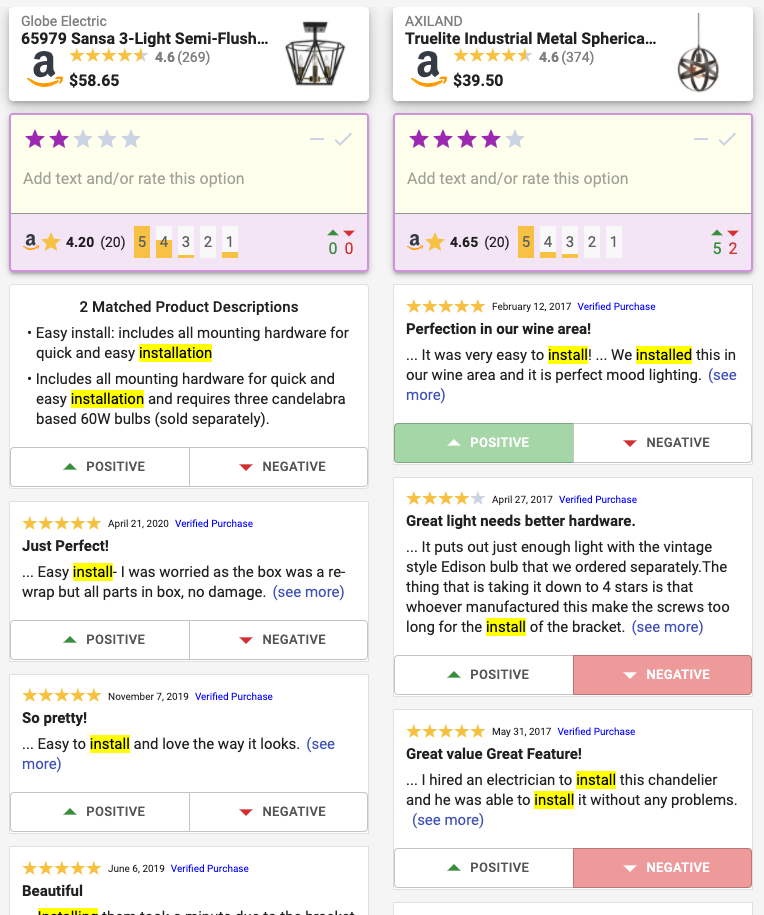
\includegraphics[width=0.7\columnwidth]{Chapters/Mesh/figures/EvidenceView_Small.png}}}
    \caption[The Evidence View for \SYSTEM.]{The Evidence View. Users can see evidence that mentioned the criteria side-by-side for their options. To capture their interpretation of evidence, users can also label reviews to build a tally or overwrite the average ratings with their own if they do not reflect their views. This is an actual project made by P05 in the field study.}
    \label{fig:EvidenceView}
\end{figure}



\subsection{[D3] Scaffolding Decision Making}

As a user iteratively builds up a better understanding of their options and criteria, they gradually progress from investigating and interpreting evidence to making a decision between their options. However, participants in the exploratory interviews described spending redundant effort when they lost track of prior judgements about options and had to revisit webpages and reread their content to remind themselves what they liked and disliked about an option. When using \SYSTEM, participants can see all their previous judgements in the Table View presented as cell values in each Option Column. This includes the review tallies and their own ratings and notes about each criteria. This allowed users to have an ``birds eye view'' of their research, seeing which criteria and options contained their own ratings and notes, decide what to focus on next, as well as seeing trade-offs between the options when making purchase decisions.

Participants in the exploratory interviews also described "analysis paralysis" when reaching the decision stage, in which many of their options looked similar on the surface (i.e., highly rated and based on hundreds of reviews) and that it can be difficult for them to see clear trade-offs on multiple criteria for their options. \SYSTEM also provided several affordances for users to interact with their options to explore the trade-offs between them towards making purchase decisions. Firstly, \SYSTEM computes an overall rating for each option by averaging ratings for its criteria. When averaging, \SYSTEM will use users’ own ratings when available, and default to the average Amazon review ratings otherwise. Given that participants in formative studies mentioned the importance of different criteria having differing weights in their decision making, the system also enables them to specify the weight for each criteria which correspondingly alters its impact on the weighted average (e.g., a 5x weight will be counted 5x towards the weighted average more than the default 1x weight). \footnote{Details of this calculation is explained to the users via a hovered tooltip. Checks and missing symbols were counted as 1 and 5 stars, respectively.} We also supported ``soft'' prioritization by enabling users to freely reorder rows and columns via drag-and-drop, for example, to move the most promising options or criteria to the top or the left without altering the overall score. Finally, \SYSTEM could also sort options based on individual criteria ratings or the overall ratings when users click on the sort icon next to the criteria names. This allowed users to quickly explore the best and worst performing options based on their criteria. 


\section{Evaluation}

We conducted three studies that focused on exploring the following research questions, respectively:

\begin{itemize}
  \setlength\itemsep{0em}

\item The usability of our implementation and the benefits of gathering and presenting evidence across sources. (Study 1)

\item Does \SYSTEM enable users to gain more insights from data compared to Google Spreadsheets? (Study 2)

\item What are the longer term effects of deploying \SYSTEM to users conducting their own personal tasks? (Study 3)
\end{itemize}

The first two studies were controlled studies comparing \SYSTEM to a baseline condition using predefined tasks to control for task complexity. Participants were recruited from Amazon Mechanical Turk who had more than 100 accepted tasks with above 90\% acceptance rate and lived in countries that primarily spoke English. Due to the limitation running Mechanical Turk studies, we could not install \SYSTEM on their computers as a Chrome extension. We therefore deployed the same system as a hosted webpage for participants to interact with. The third study is a field deployment in which participants installed \SYSTEM on their own computers (as a Chrome extension) and conducted their personal tasks over a longer period of time. Participants for the field study were recruited from the local population primarily by posting to discussion boards on NextDoor, a neighborhood based social media. We used video conferencing and screen sharing softwares to assist with the installation process and to conduct two rounds of interviews.

\subsection{Study 1 - Usability Test and Interaction Costs}


The main goals of our first study was to verify in a controlled environment the usability of the \SYSTEM and to test if the mechanism of automatically pulling in evidence from different information sources can allow users to work more efficiently and find more accurate information. For this, we compared \SYSTEM to a baseline variant as a within subject condition where evidence was not automatically pulled in and used objective criteria that had gold-standard answers so we can measure the accuracy of participants’ responses. During the baseline condition, participants can use any strategies based on their own product research experiences, such as searching for keywords on Amazon product pages and/or use search engines to find more sources. In order to measure how effective participants were in finding the right answers, we used fixed product options (i.e., 5 popular espresso machines on Amazon) and objective criteria.\footnote{Dimension, Does it have a built-in grinder, Water tank size, Does it use a solenoid valve and Portafilter size} One of the authors compiled the gold-standard answers before running the study. Almost all answers were obtained from the manufacturer’s website (such as in specification tables and downloading PDF user manuals), with a few resorting to using expert reviews (namely photos or videos that showed a measurement of the portafilters).

The goal of the main task was to find the correct answer for each criteria for the given options. The criteria cells for the first options were filled out to serve as an example. The study was broken down into two segments, and participants worked on two of the four remaining options during each segment with a different condition (counterbalanced for order). During the \SYSTEM condition, evidence was gathered from Amazon reviews and product descriptions, as well as the top two product review webpages returned from Google when searching with the product names appended with the term “reviews''. Links to the same sources were also presented during the baseline condition. During the study, we recorded the time each participant spent in the two conditions as well as their responses. After the study, we used the NASA-TLX survey to collect their perceived workload for each of the two conditions. A total of 24 participants were recruited from Amazon Mechanical Turk (age 21-68 M=36.8; SD=10.5; 15 males and 9 females).  Each participant was compensated 3 US dollars for an average of 24.9 minutes (median=22.7, SD=8.3).

\subsubsection{Study 1 Results}



\begin{figure*}
    \centering
    \textcolor{gray}{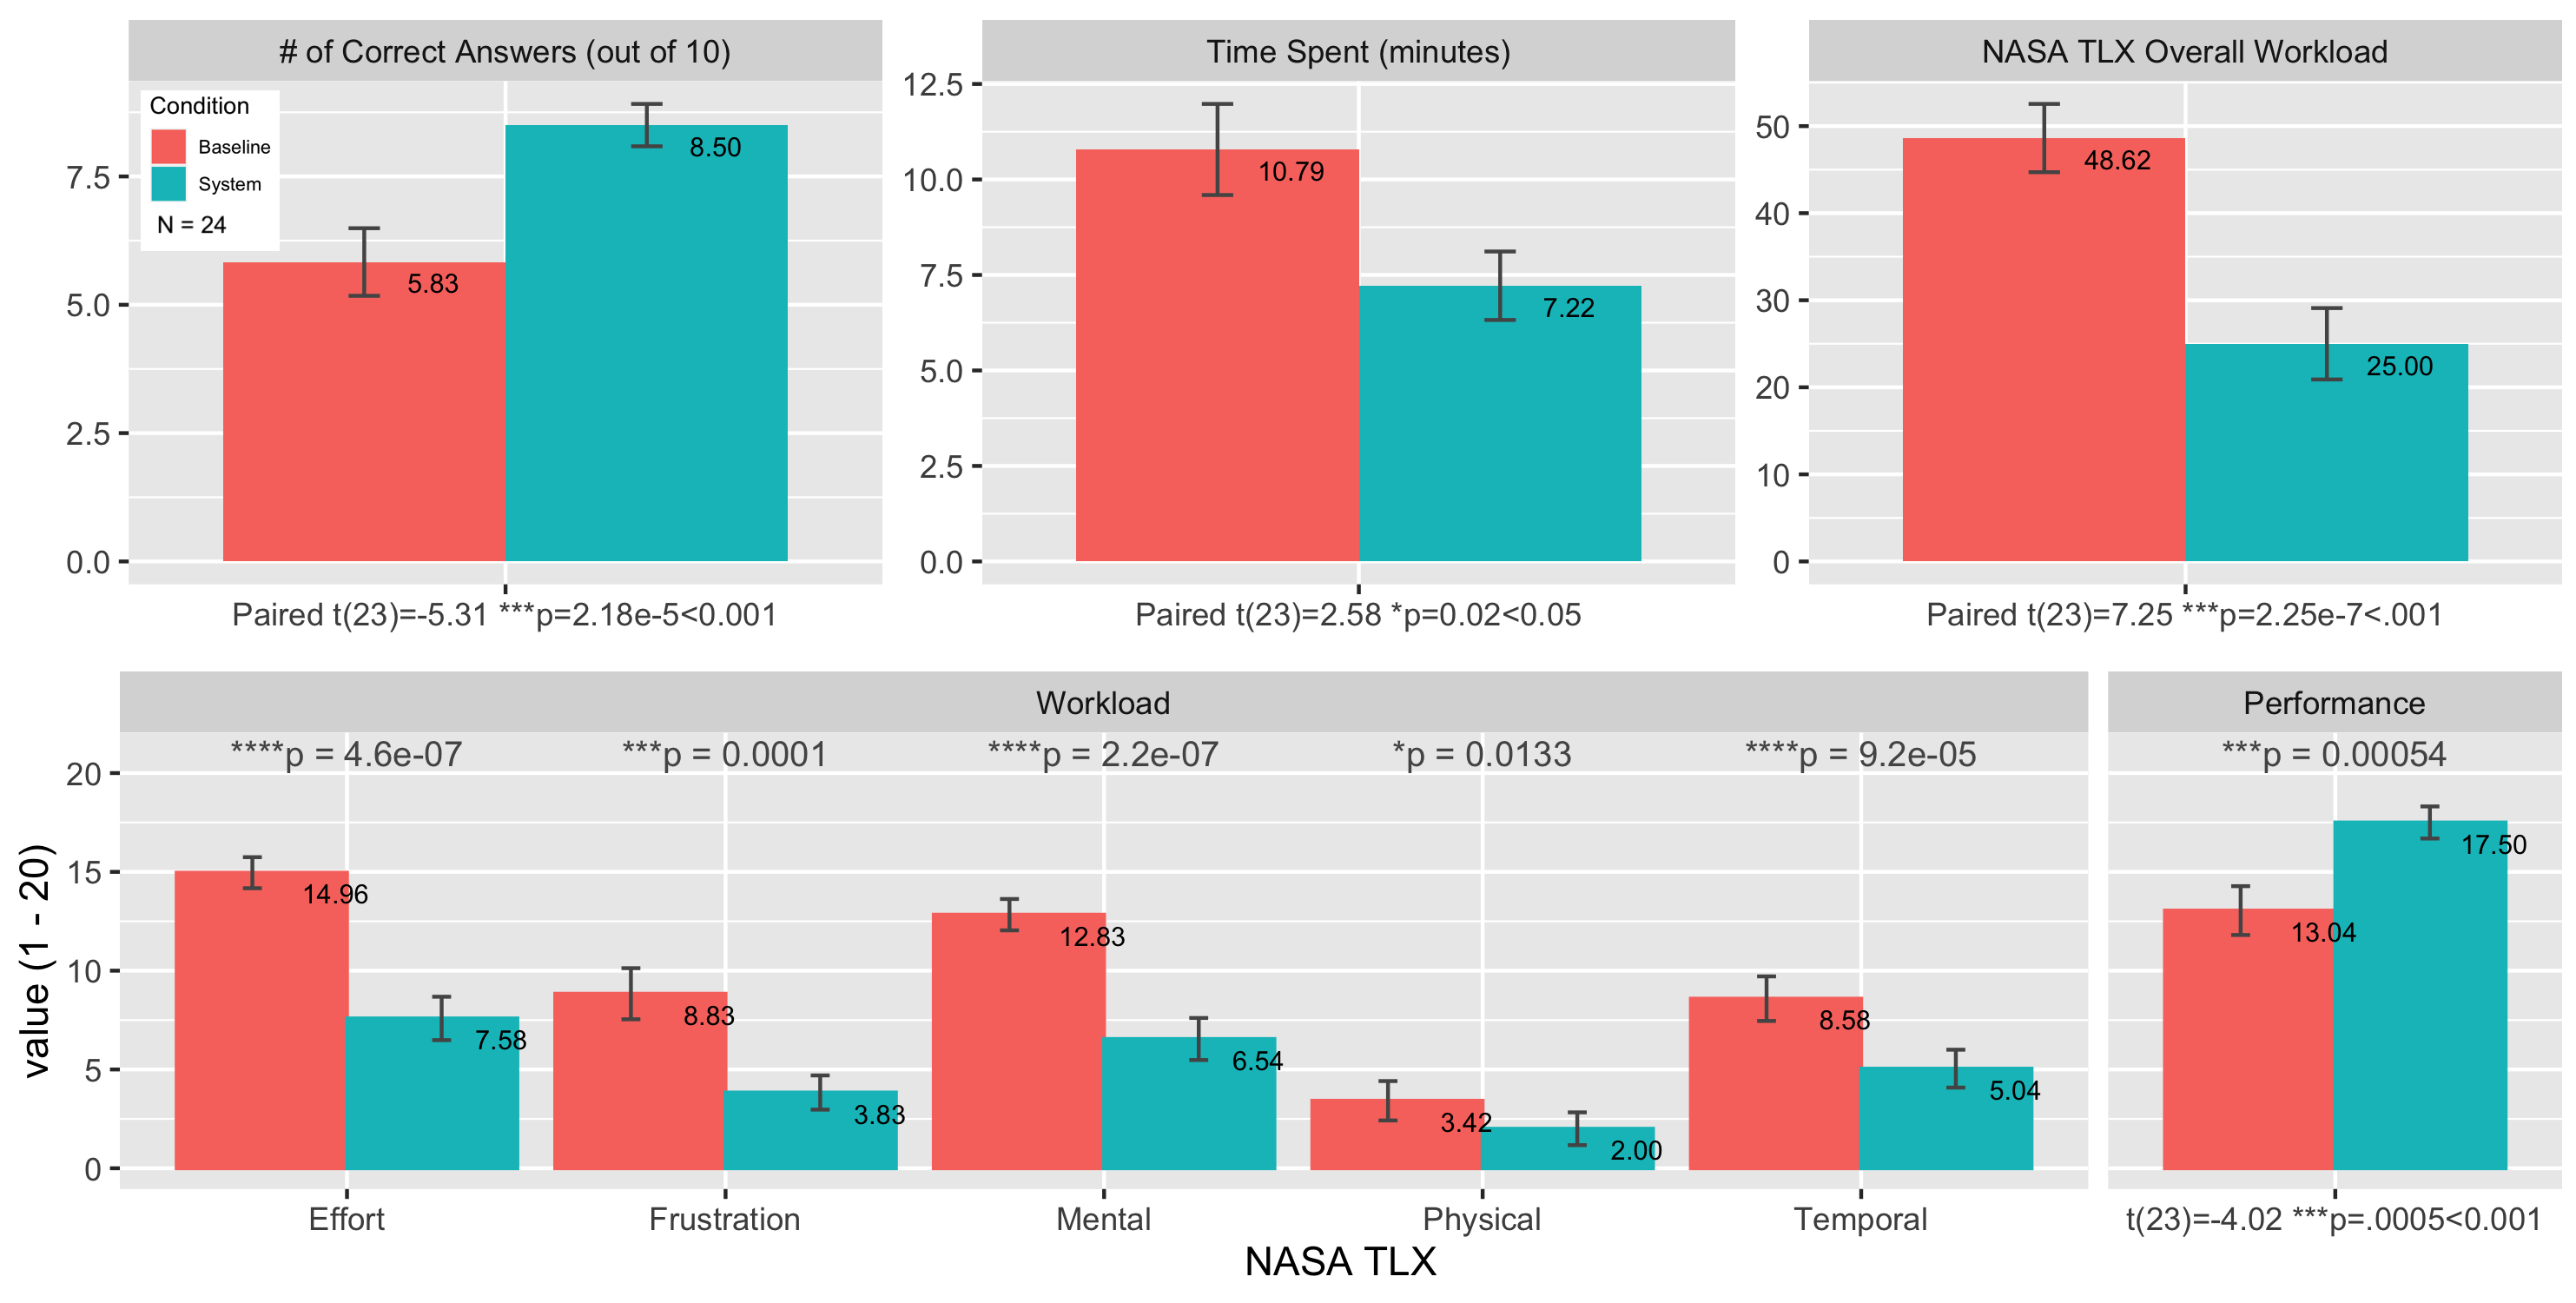
\includegraphics[width=1\textwidth]{Chapters/Mesh/figures/Interaction.png}}
    \caption[Mean statistic for the objective criteria study.]{Mean statistic of how participants performed under different conditions. Participants who used \SYSTEM were finding more correct answers using a shorter period of time. In addition, they also had lowered perceived workload based on the NASA-TLX survey.}
    \label{fig:interaction}
\end{figure*}


Results suggest that the 24 participants performed the given task more efficiently when in the system condition than when they were in the baseline condition. Comparing \SYSTEM with the baseline, participants completed their tasks faster when using \SYSTEM that gathered evidence automatically across multiple sources (7.2 vs 10.8 minutes; t(23)=2.6, *p=0.017<0.05 based on a paired t-test). At the same time, they found information that were more accurate based on gold-standard answers (85.0\% vs 58.3\%; t(23)=-5.31, ***p=2.18e-05<0.001 based on a paired t-test). Combining the two metrics we estimated a x2.30 increase in efficiency, where participants were finding 2.23 correct answers on average each minute when using the full \SYSTEM system, compared only 0.97 correct answers per minute on average when using the baseline variant (based on a paired t-test: t(23)=4.18, ***p=0.00036<0.001).

In addition to speed and accuracy, participants also perceived the process to have lowered workload when using the full system across effort, frustration, mental, physical and temporal demands based on the NASA-TLX survey (Figure~\ref{fig:interaction}, combined: 25.0/100.0 vs 48.6/100.0; t(23)=7.25 ***p=2.25e-7<0.001 based on a paired t-test)  as well as increased perceived performance (17.5/20.0 vs 13.4/20.0; t(23)=-4.02, ***p=0.0005<0.001 based on a paired t-test). This suggests the interface of \SYSTEM can reduce interaction costs when dealing with objective criteria when compared to the baseline where participants relied on their current process, even when they had to learn a new interface.



\subsection{Study 2 - Interpreting Subjective Evidence}

While the first study tested the usability and interaction costs of \SYSTEM when working with objective criteria with gold-standard answers, Study 2 focused on how \SYSTEM can support users when investigating criteria that required subjective and potentially messy and conflicting evidence such as consumer reviews\cite{hoch1986consumer}. Unlike looking up the product dimensions in the product description for a coffee machine, investigating its ease of use may require users to read through multiple relevant reviews to get a sense of how previous consumers agreed or disagreed on the criteria while considering how each review fits their personal context. For example, a user buying a robot vacuum who lived in an apartment with wooden floors might down-weight reviews from people who lived in a big house with high pile carpet. For this, we carried out a second study that focused on whether \SYSTEM can provide benefits when researching these types of subjective criteria. 

To compare \SYSTEM with people’s existing approach, we used Google Spreadsheets as a between subject baseline. We chose this baseline because it is a common tool for consumers building product comparison tables, and that it is an easily accessible hosted service with APIs that allows us to dynamically create a spreadsheet for each crowdworker. To control for task complexity and the personal preferences of participants, we used the following persona and task description for researching 5 robot vacuum cleaners with the 3 subjective criteria in bold: 

\begin{tightquote}
John is looking to buy a robot vacuum for his house. The most important thing for him is that the robot vacuum \textbf{doesn't get stuck too often}. It is also important that it is \textbf{not too loud}. He also has a dog, so it would be nice if it's also \textbf{effective cleaning up dog hair}.

John already narrowed down to 5 final options. Spend around 20 minutes to build up a comparison table to help John research the best option and explain to him why you think it is the best option.
\end{tightquote}

\begin{figure}
    \centering
    \textcolor{gray}{\frame{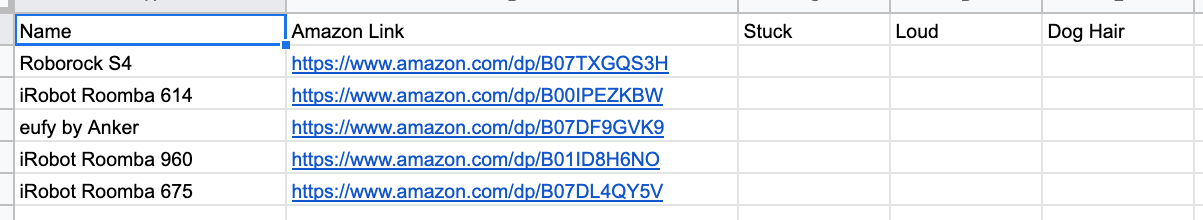
\includegraphics[width=0.8\columnwidth]{Chapters/Mesh/figures/baseline_sheets.png}}}
    \caption{The initial spreadsheet for the baseline condition.}
    \label{fig:baseline}
\end{figure}

The five options were all popular models on Amazon that had more than 1,000 reviews and above 4 average review ratings (as of April 15, 2020). In both conditions, we populated their tables with the predefined options and criteria to maximize the time participants spent on exploring and learning from data instead of copying and pasting information from the persona (see Figure~\ref{fig:baseline} for the baseline template).

A total of 48 unique participants from Mechanical Turk for the main study. In which 22 (age 31-58, M=38.7, SD=9.6) were randomly assigned to use \SYSTEM and the remaining 26 participants (age 30-70, M=34.7, SD=11.3) used Google Spreadsheet. Each participant was instructed to conduct the above task for 20 minutes using their assigned systems. We assumed participants in the baseline condition to be already familiar with a spreadsheet interface, and gave a brief tutorial (13 sentences and 6 screenshots) to participants assigned to use \SYSTEM. To capture what participants had learned during 20 minutes of research, we asked them to pick one of the options that they recommend and write a short summary for John explaining their choices. This design allowed us to capture the mental models of participants under different conditions through mentions of detailed evidence and how they reasoned and compared the different options, and has shown to be effective for evaluating sensemaking support systems in prior work \cite{kammerer2009signpost,nelson2009little}. Workers who participated in the previous study were excluded from this study to prevent learning effects. Each participant was compensated 3 US dollars. 

To compare summaries collected from the two conditions, each summary was rated by 5 additional crowdworkers. Crowdworkers who participated in the Study were excluded to ensure summaries were not rated by the participants who wrote them. In each rating task, crowdworkers first read the same persona used in the study and one of the summaries. Crowdworkers then rated rated the following statement using 7-point Likert scales for agreement (a score of 7 indicated a strong agreement, a score of 1 indicated a strong disagreement), and we averaged the ratings across 5 workers as the final ratings:

\begin{itemize}
  \setlength\itemsep{0em}

    \item I find the summary to be \emph{useful}.
    \item The summary is \emph{relevant} to the scenario.
    \item The summary is \emph{insightful}, containing details that may be hard to find.
    \item I feel \emph{confident} after reading the summary.
\end{itemize}

The four statements were designed to compare the summaries across conditions on the following aspects: The first statement of usefulness aimed to measure their quality to account for collecting qualitative responses on crowdsourcing platforms \cite{kittur2008crowdsourcing}. The second statement measured whether participants who used \SYSTEM were able to focus on criteria described in the persona and generate summaries that were more relevant.  This is due to the fact that participants in our fact-finding study described their current process as ``\emph{a rabbit hole}'' and how it can be difficult to ``\emph{focus on criteria that really mattered}.'' The third statement measured how detailed and insightful the summaries were, an important aspect of consumer review helpfulness identified in a prior work \cite{mudambi2010research}. Finally, the fourth statement aimed to explore whether information in the summaries can support decision making by measuring if they induce confidence. 

Workers were paid 0.25 cents for reading the persona and rating summary based on the four statements above. \footnote{Workers read an average of 124.0 words for each task (range: 50.0-220.0, SD=44.4) and the estimated reading speed of English speakers is 200-300 words per minute \cite{siegenthaler2012reading}. Assuming the lower-bound reading speed of 200 words per minute and 15 seconds was required to answer each of the four Likert-scales. Similar to approach in \cite{10.1145/3313831.3376715}, we estimated the average hourly pay rate to be around 9.26 USD.} 


\subsubsection{Study 2 Results}

\begin{figure*}
    \centering
    \textcolor{gray}{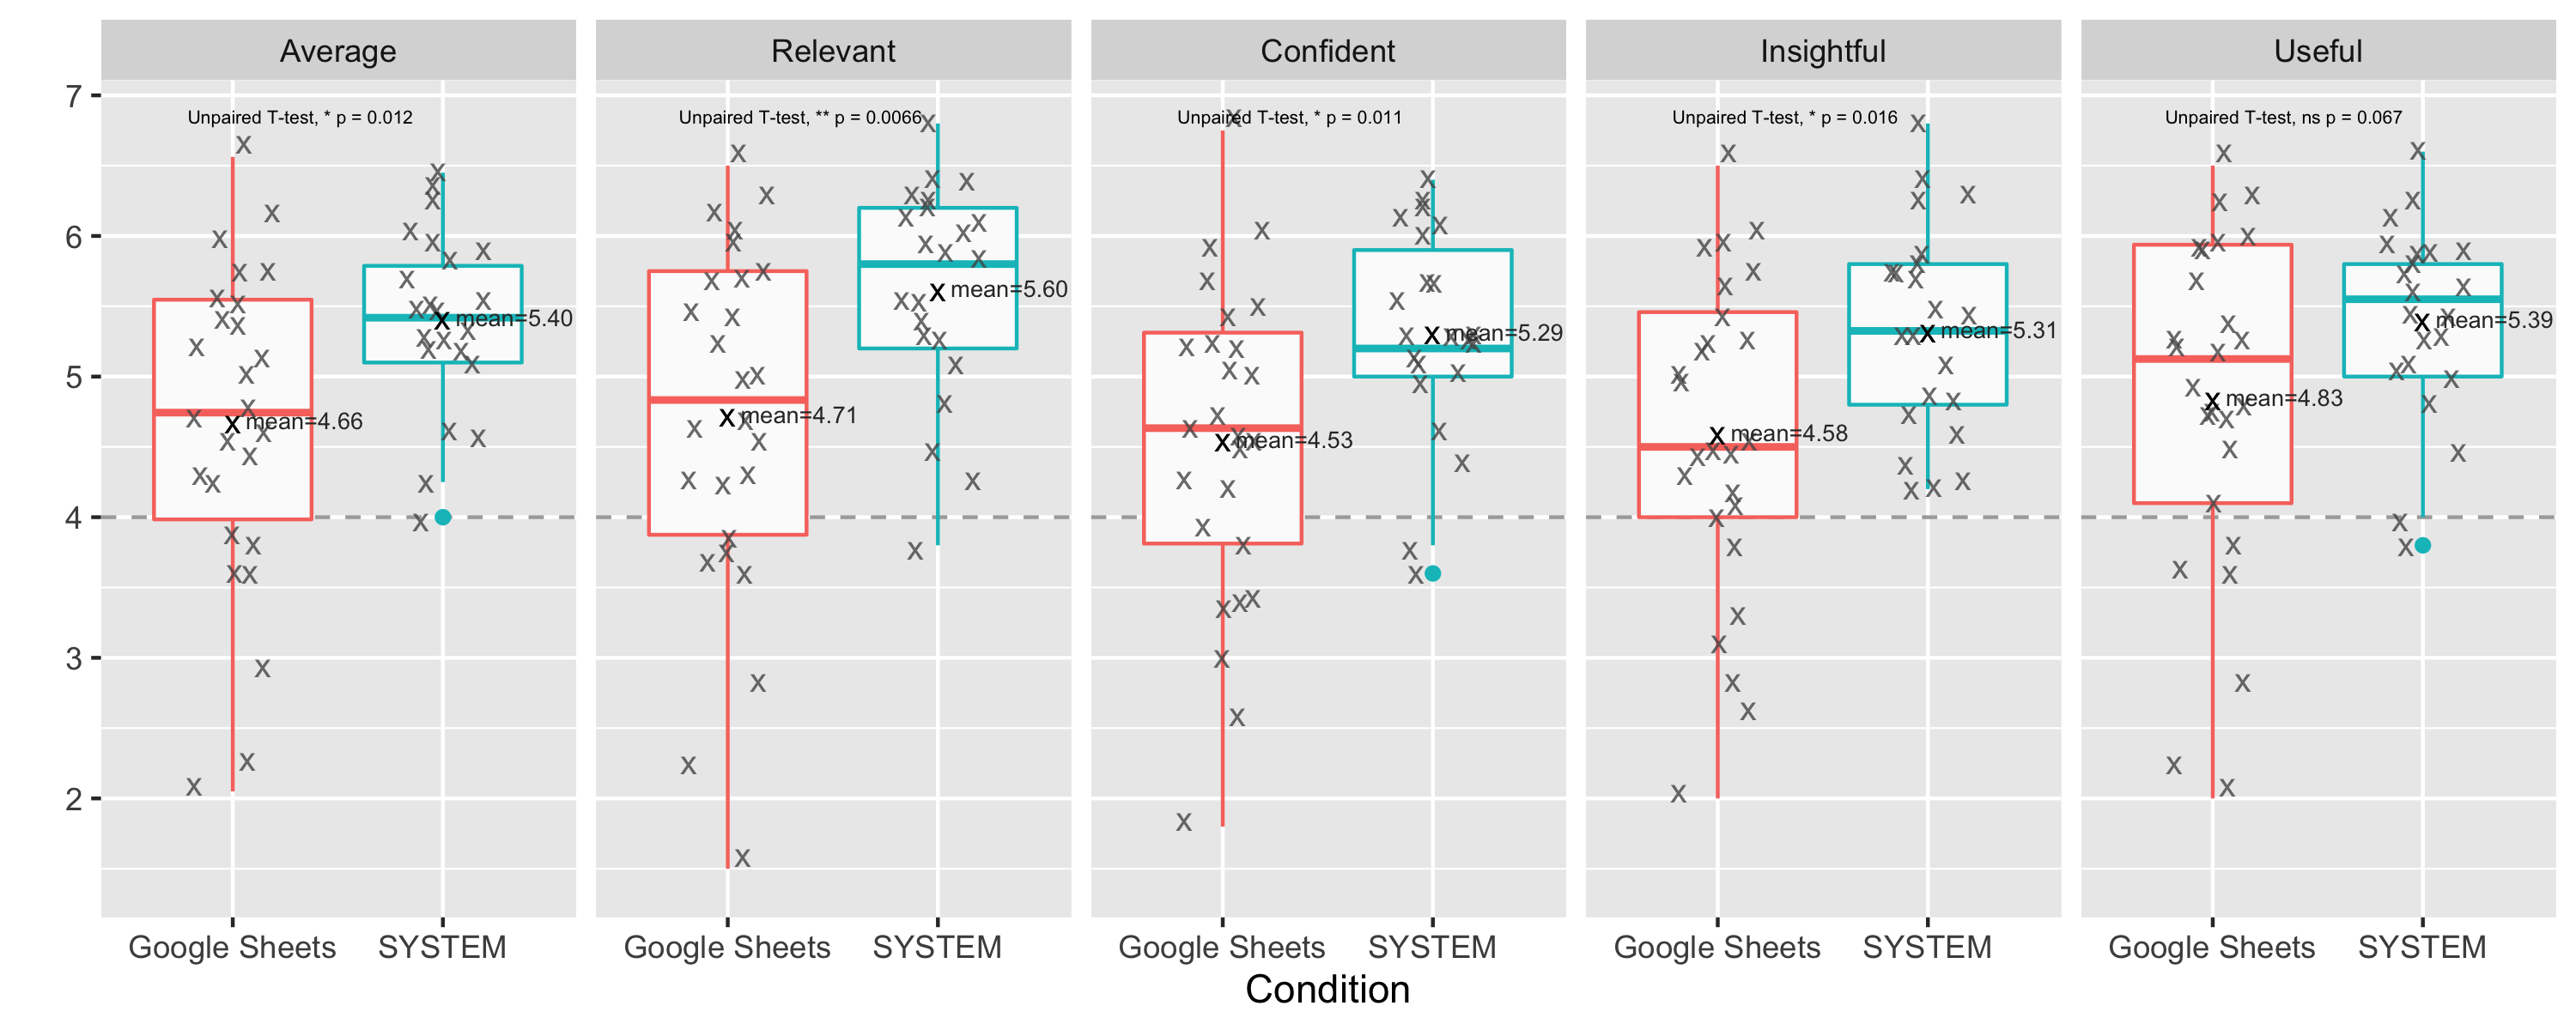
\includegraphics[width=1\textwidth]{Chapters/Mesh/figures/Subjective.png}}
    \caption[Mean statistics for the subjective criteria study.]{Using a 7-point Likert-scale for agreement where 4 is neutral and a MANOVA, we that participants who used \SYSTEM generated learning summaries that were rated significantly higher compared to participants who used Google Sheets for the same task on the combined dependent variables of  relevance, confidence, insightfulness, and usefulness (F(4, 43)=2.64, *p=0.047<0.05).}
    \label{fig:subjective}
\end{figure*}

Figure~\ref{fig:subjective} shows the differences between the 22 summaries written by participants using \SYSTEM and the 26 summaries written by participants using Google Spreadsheets for the same task. Averaging across the four aspects, participants who used \SYSTEM generated summaries that were rated higher than participants in the baseline condition (Figure~\ref{fig:subjective}, mean 5.40 vs 4.66). We used a MANOVA to correct for multiple comparisons and found statistically significant difference (F(4, 43)=2.64, *p=0.047<0.05) between the conditions on the combined dependent variables (relevance, confidence, insightful and usefulness). Below we show two typical summaries from each of the conditions collected after 20 minutes of product research:

\begin{tightquote}
\textbf{Baseline condition}: I would pick the Roborock S4 after considering the 3 categories [criteria] that are important to him: how often it gets stuck, noise, and ability to pick up hair. Unfortunately, all of the models he picked do have a tendency to get stuck, which makes it difficult to choose when just using the three factors [criteria]. However, the Roborock was the only model I found, where there weren't many complaints about it being too loud. Additionally, the Roborock is able to pick up dog hair, according to the product description and user reviews.

\textbf{System condition}: It seems that while all options do tend to get stuck from time to time, the reviews that the Roomba 675 does somewhat better in that regard. Additionally, many reviews for the Roomba 675 stated how well it picks up pet hair, which was another important consideration that differentiated the Roomba 675 from other options. The Roomba 960 may be marginally better but it costs \$200 more and so I didn't think it was worth the extra expense. Lastly there were reviews that found the noise of the Roomba 675 to be acceptable. 

\end{tightquote}

While many participants who used Google Sheets mentioned the similarity between options and the difficulty of the task, people who used \SYSTEM point out how they differentiated the options on the given criteria based on multiple pieces of evidence. 

\begin{table*}
  \centering
  \small
% question, number of sources, number of clips, number of turkers
  \begin{tabular}{ l l l l}
  
	\hline
	
	\textbf{ID} & \textbf{Tasks} & \textbf{Minutes Spent} & \textbf{\# of Sessions} \\
	
	\hline
	
	P01 & Snow boots. Gourmet cat food. & 70 & 3 \\
	P02 & Backpacks. Pajamas as a gift for his/her sister. & 134 & 3 \\
	P03 & Bread machine. Hair cutting kit. & 150 & 4 \\
	P04 & Running shoes. Printer for learning material for kids. & 82 & 6 \\
	P05 & Entryway light fixture. Toy play-set for kids. & 131 & 5 \\
	
	\hline
	
  \end{tabular}
  \caption[List of participants and usage pattern for the deployment study.]{Usage statistics about participants in the field deployment study based on the activity logs. This includes the tasks they conducted using \SYSTEM, as well as the total number minutes they spent using the system and the number of sessions over the deployment period.}
  \label{tab:participants}
\end{table*}

\subsection{Study 3 - Field Deployment Study}

While the first two studies provided quantitative measures on how \SYSTEM affected learning, efficiency, accuracy and perceived workload when participants were given predefined tasks, we also conducted a field deployment to further investigate the longer term effects of \SYSTEM when participants performed their personal tasks in the wild. Five participants (age: four 25-34 and one 35-40; two females, two males and one non-binary) were recruited by posting to 5 local neighborhood discussion boards on NextDoor (a neighborhood based social media website). The posts contained a link to an online screener survey, and we used the responses to recruit to people who have used a spreadsheet for online research in the past (49.4\%, N=89) and prioritized people who had any Chrome extensions installed (49.4\, N=89). 

We interviewed participants for one hour at each the beginning and the end of the deployment. Before the initial interview, we asked each participant to email us 1 to 3 upcoming online purchases to ensure they have a real task to work on during the initial interview. At the start of the first interview, we collected their demographic information and assisted with installing \SYSTEM as a Chrome extension on their computers via screen sharing. Each participant then proceeded to perform a think aloud session for around 30 minutes using \SYSTEM to conduct one of the tasks they had proposed. After the first interview, participants continued to use \SYSTEM on their own for the same tasks and/or create new tasks. Based on their availability, we interviewed each participant again after 1-2 weeks. Participants shared their screens and retrospectively walked us through their projects while we probed on their experiences, strategies and issues they had encountered during the deployment. Table~\ref{tab:participants} shows the tasks each participant conducted and the total amount of time they spent using \SYSTEM based on log data. The first tasks in the table were ones created during the initial interview and the rest created during deployment. All 5 participants completed the study and were each compensated a 50 US dollars Amazon gift card. The interviews were video recorded and transcribed for analysis.

\subsubsection{Study 3 Results}

Following an open coding approach based on grounded theory, the first author went through the 10 hours of recordings and transcriptions in three passes, and iteratively generated potential categories from the dialogue until clear themes emerged \cite{charmaz2007grounded}. Throughout the iterations, inputs from the rest of the research team were also incorporated, including other researchers who also conducted interviews. Our key findings are presented below.

\emph{\underline{Efficient and Organized}}

In general, participants responded favorably to using \SYSTEM in the field for their personal tasks when asked to compare \SYSTEM to their current online product research process (i.e., using spreadsheets and/or notepads). Specifically, all participants pointed to lowered interaction costs when using the Evidence View to access evidence gathered across information sources to compare their options, as well as lowered cognitive costs from being able to rule out options confidently based on evidence.

\begin{tightquote}
 
It is much better than a spreadsheet... I like that I can really quickly add something and it just pulls in all the information, the picture, the price, and [evidence for] all of these different criteria and presents it in a way that is really easy to do comparison across products. I'm able to delete things easily so that I can reduce my cognitive load as I go through my decision making process. - P03

\end{tightquote}

All participants described how \SYSTEM allowed them to take a more organized and structured approach when managing multiple information sources and foraging evidence from them. Specifically, P01 and P02 described how the linear structure of browser tabs can be inefficient when trying to find evidence for a specific criteria across browser tabs for different options. While participants also pointed out that the mechanisms provided by \SYSTEM can technically be performed manually, they also acknowledged that the interaction costs of managing many browser tabs and filtering for relevant information to support their criteria amongst them would be prohibitively high in practice.

\begin{tightquote}

In theory I could do all this myself but it would take 10 times [as] long so I would never do it well. I would say is it technically possible? Yes. But would any person ever do this [manually] for themselves? ...  It's nice to have a more organized and systematic approach… Instead of something that right now is very linear. If I pulled up a bunch of boots in different tabs and searched [in] each of them for reviews with the word boar. It's really boring and not a particularly efficient way to look at information. - P01

\end{tightquote}

One participant (P03) pointed to how having a more organized scaffold to their processes, \SYSTEM provided better support task resumption, allowing them to make progress on their overall tasks even with shorter sessions.

\begin{tightquote}

I loved being able to come back to this [referring to one project]. It's something we hadn't done in our initial sessions that became so much better when I was using it on my own. I couldn't say, hey, I've got 15 minutes to kill. Let me do some more searching, and then I could say, okay, gotta go to my next meeting. - P03

\end{tightquote}

Post-analysis based on activity logs also found all participants conducted their product research in three to six sessions (Table~\ref{tab:participants}).

\emph{\underline{Prioritizing Effort on Discriminative Criteria}}

We found two major usage patterns for the criteria-specific average Amazon ratings, both centered around being able to discover discrepancies between participants’ options.  All participants saw immediate value when the average Amazon ratings populated automatically for their options when they added a new criteria. Allowing them to get an initial overview of how the evidence differs between options for a criteria. Specifically, participants described trying out different criteria as a way to surface meaningful differences (i.e., based on their own criteria) amongst their options. Since participants typically only considered options that were popular and highly rated on Amazon, they described their options as virtually indistinguishable without \SYSTEM:

\begin{tightquote}
Having never purchased it before I literally have no idea what to buy. And so this [task] is what I tried to do [with \SYSTEM] and it's actually like super helpful because [otherwise] every single stupid cat food on Amazon just like looks identical…So, it was really helpful especially [with] this picky criteria. - P01

\end{tightquote}

Alternatively, when participants added a new option to a project that had existing criteria, \SYSTEM automatically populated Amazon average review ratings across different criteria for the new option. Participants used this mechanism to quickly characterize new options and see how they fit with existing options based on their own criteria:

\begin{tightquote}

But now, you put this kind of data in front of me in this quick hit fashion. Then I go, wow! They're pricey [comparing a newly added option to existing ones], and yet anybody that mentioned cost [a criteria] has given it the full rating. They're more durable [referring to discrepancy between options in the average ratings for a criteria] You know, I could see tangible evidence now. And that makes me want to go -- Maybe that's the pair.  - P04

\end{tightquote}

Seeing discrepancies between options also influenced participants’ process by prompting them prioritize their effort on investigating criteria that had large discrepancies between their different options:

\begin{tightquote}

Okay, there wasn't a great difference here in terms of ink [a criteria]. Let me go into what I weighted as more important, and it's this air printing [another criteria] capability… for this middle one [referring to one option], rated pretty poorly… These two have pretty good ratings. So then I went in and started looking [at the evidence] - P04

\end{tightquote}

By focusing first on criteria that were more discriminative amongst the options, participants could rule out options that compared less favorably earlier to shortcut their process. All participants described prioritizing their options in the system, either by reordering their options via drag-and-drop, or rule out options completely by removing them. One participant in particular, described a sense of relief and progress when removing options in \SYSTEM. 

\begin{tightquote}

I don't feel like I would delete things [options] in a spreadsheet. Whereas here it actually feels good to delete it [an option], because I'm like, Great! I've decided that I'm not going to deal with it.  - P03

\end{tightquote}

\emph{\underline{Scaffolding Decision Making}}

Participants also described how \SYSTEM supported deep exploration of individual pieces of evidence in the Evidence View that laid out evidence for specific criteria across their options.

\begin{tightquote}

The second thing that I think is really great for me was the ability to dive into the reviews for specific criteria. It's really nice to be able to open this [the Evidence View] up and have it filter out for all of the products, so I can make this comparison across products.  - P03

\end{tightquote}

When we introduced the system, we explicitly explained to participants that the average ratings were based on review scores and could be influenced by parts of a review not relevant to their criteria even though the reviews mentioned the criteria. Participants were able to work with this limitation, and replaced the Amazon ratings with their own when they do  not reflect how they wish to characterize the evidence. In addition, participants also described creating ratings as a way to keep track of and aggregate how they personally interpreted evidence and saw benefits in how changing criteria ratings was reflected in the overall weight score of each option.

\begin{tightquote}

I would say in the event that I was going to differ from what's in front of me, I would rate [the criteria]. - P04

\end{tightquote}

\begin{tightquote}

Once I start to make decisions on things, like I put my thing [own ratings and notes] in there and say: Okay, this is what my rating is. And now it starts to change the overall ratings, so it would help me make a better decision based on what I think…. like, the tool thinks this is a really good value, but maybe I think this value is not enough for me and it's a two, because I just think it's two - P03

\end{tightquote}

All of the participants also made actual purchases during the deployment based on their research performed with \SYSTEM and expressed confidence in their decisions. This suggests that their tasks represented real world user needs, and our participants were able to use \SYSTEM to conduct research for a prolonged period of time and use it to support making their final purchase decisions.


\section{Discussion and Limitations}


While all participants’ initial responses were positive when adding options and criteria to the Table View, some of them find their first impressions of the Evidence View to be overwhelming. While this suggested a higher learning curve for the Evidence View, all participants were able to complete research with it for their own tasks during the deployment.

\begin{tightquote}
So initially it was like, Whoa, there's a lot going on here. It's a lot of text but I'm kind of over it  once I understood what was going on. Now I'm like, Okay, cool. Let's take a look at this [referring to the criteria] across the things [referring to the options] - P03
\end{tightquote}

More commonly, participants express desire to extract evidence from online sources other than Amazon. While in the current implementation does support extracting evidence from other sources through pasting in their URLs to the appropriate option, participants pointed to two limitations: 1) extracting and tracking price changes across ecommerce platforms other than Amazon and be notified, and 2) extracting from listicles and forum posts that discussed multiple products: 

\begin{tightquote}

Running shoes are kind of discipline specific. There are other sites solely for this [type of] product that I would go to. [To add a webpage and] track the options to use globally would be cool. But like robot vacuum there's nowhere else [but Amazon] I'm going. Unless I'm tipped off that Target or Bed Bath and Beyond happened to have an incredible sale. - P04

\end{tightquote}


While price tracking could be implemented within \SYSTEM, there are multiple commercial solutions available \footnote{https://camelcamelcamel.com/ and https://www.joinhoney.com/} and we considered it outside the scope of this work. On the other hand, extracting information from sources containing evidence about multiple options presents an interesting research challenge of computationally identifying mentions of products and extracting descriptions about them from text. 
Finally, in our design we relied on the users to generate the list of options and criteria. While recommender systems or aspect extraction techniques could also be incorporated into the system to support this in the future, many were already commercially available on ecommerce platforms which also potentially explain why this was not a salient issue in the interviews.

%\section{CONCLUSION}

We introduced \SYSTEM, a novel system where users to build up product comparison tables connected to information sources as a way to scaffold their research. This design is novel because it introduced a new process that scaffolds the building up of context and changes the cost structure from increasing cost to increasing payoffs as the number of criteria and options grow. Through three rounds of lab and field studies, we gained deeper insights into how \SYSTEM can benefit online sensemaking in the context of product comparison research. We found evidence that \SYSTEM not only lowered the interaction costs (i.e., faster and lowered perceived effort) by pulling in information across sources about objective criteria (e.g., the water tank capacities for different espresso machines), but also allowed participants to find more accurate information (Study 1). When dealing with subjective criteria (e.g., ease of use for different espresso machines), we found evidence that participants who used \SYSTEM were more insightful and confident about their choices compared to participants who used Google Spreadsheet in the baseline condition (Study 2).  We also tested \SYSTEM in the wild with participants conducting their own tasks over a longer period of time. Post-interview revealed insights on how \SYSTEM allowed them to prioritize their investigation on criteria that were discriminative amongst the options they were considering, enabled them to keep track of their progress by capturing their own interpretation of data, and allowed them to make confident purchases based on their findings (Study 3). 





% BALANCE COLUMNS
\balance{}
